\chapter{FACT}
\begin{wrapfigure}[24]{R}[0pt]{0.50\textwidth}
  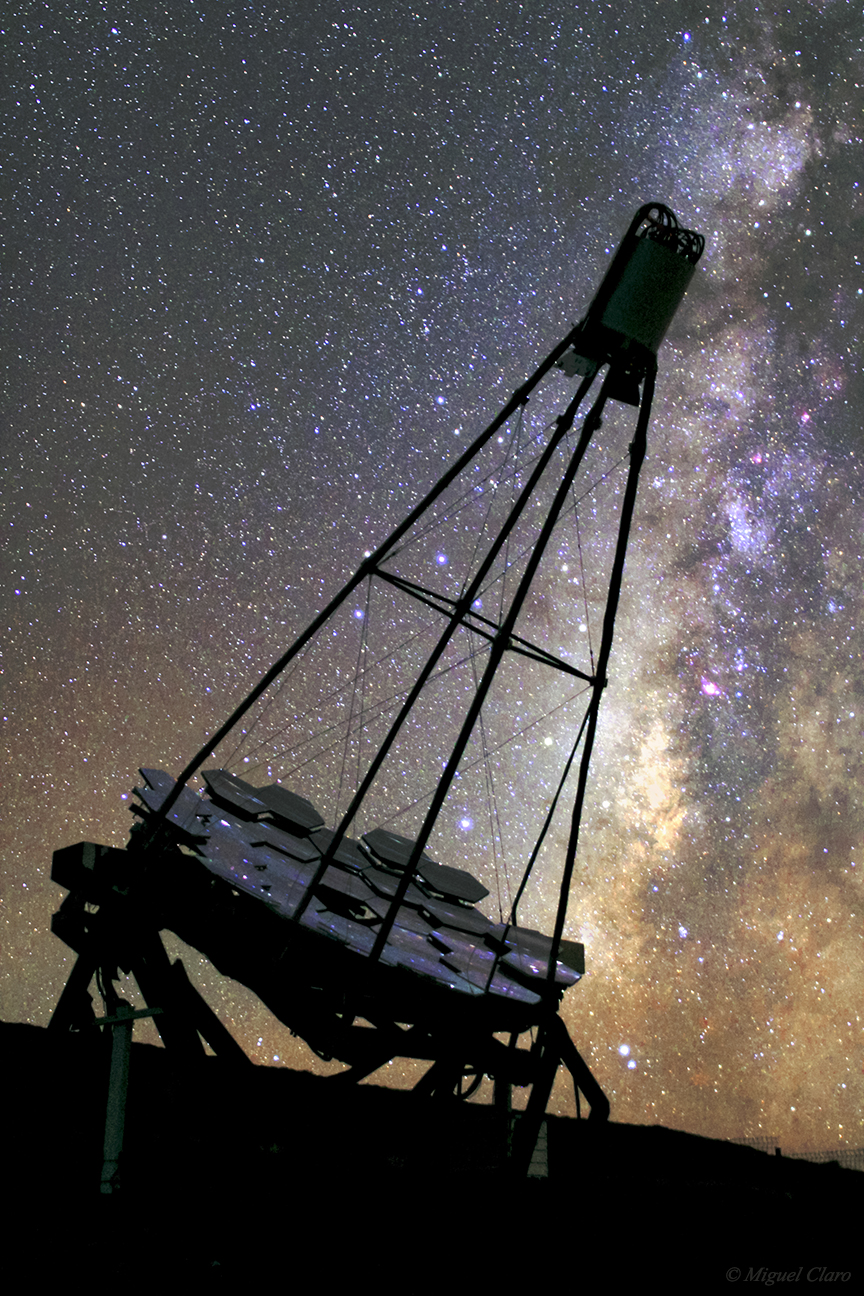
\includegraphics[width=0.50\textwidth]{./images/FACT.jpg}
  \caption{FACT während der Beobachtung.\cite{factpic}}
  \label{fig:observ}
\end{wrapfigure}
FACT (First G-APD Cherenkov Telescope) dient der Überwachung von $\gamma$-Quellen, um bei erhöhter Aktivität für genauere Observationen größere Telekope zu informieren. 
Des weiteren erprobt das Teleskop die Nutzung von Silizium Photomultipliern (SiMPs), mit welchen es möglich ist, auch in Nächten mit starker diffuser Hintergrundstrahlung Quellen zu observieren. 

FACT befindet sich auf der kanarischen Insel La Palma auf einer Höhe von 2200 Metern über dem Meeresspiegel.
Das Projekt entstand als ein Nachfolgerexperiment des HEGRA CT3 Teleskops, wobei dessen Komponenten aufbereitet und wiederverwertet wurden.

Die 30 hexagonalen Spiegel bilden eine Gesamtspiegelfläche von \SI{9.51}{\meter\squared} bei einem Blickfeld von \SI{4.5}{\degree}. 
%wie sind die Spiegel denn ausgerichtet?

Als erstes Teleskop verwendet FACT SiPMs anstelle von Photomultiplier Tubes (PMTs). 
Halbleiterdetektoren lassen sich mit einer geringeren Operationsspannung (\SI{<100}{\volt}) betreiben und sind preiswerter als Photomultiplier, was sowohl die Gestaltung des Kameradesigns als auch die Finanzierung vereinfacht. 
SiPMs sind aufgrund ihrer hohen Sensitivität dazu in der Lage, einzelne Photonen zu detektieren. 
Des weiteren besteht mit FACT auch bei Vollmond noch die Möglichkeit verwertbare Ergebnisse zu produzieren.
Die Kamera besteht aus 1440 Pixeln, welche jeweils aus einem quadratischen Sensor und einem Plexiglasleiter bestehen. Die einzelnen Oberflächen der hexagonal zulaufenden Plexiglasleiter bilden dabei die empfindliche Detektionsfläche.

\chapter{Entstehung von Tscherenkow Schauern}
\label{sec:cherenkov}
Trifft ein hochenergetisches Teilchen auf die Atmosphäre, löst dieses einen Schauer von Sekundärteilchen aus. 
Die Energie der erzeugten Sekundärteilchen ist stets geringer als die der einfallenden Primärteilchen. 
Dabei wird zwischen zwei verschiedenen Arten von Schauern unterschieden. 
\begin{figure}[H]
  \centering
  \begin{subfigure}[t]{0.49\textwidth}
  	\centering
	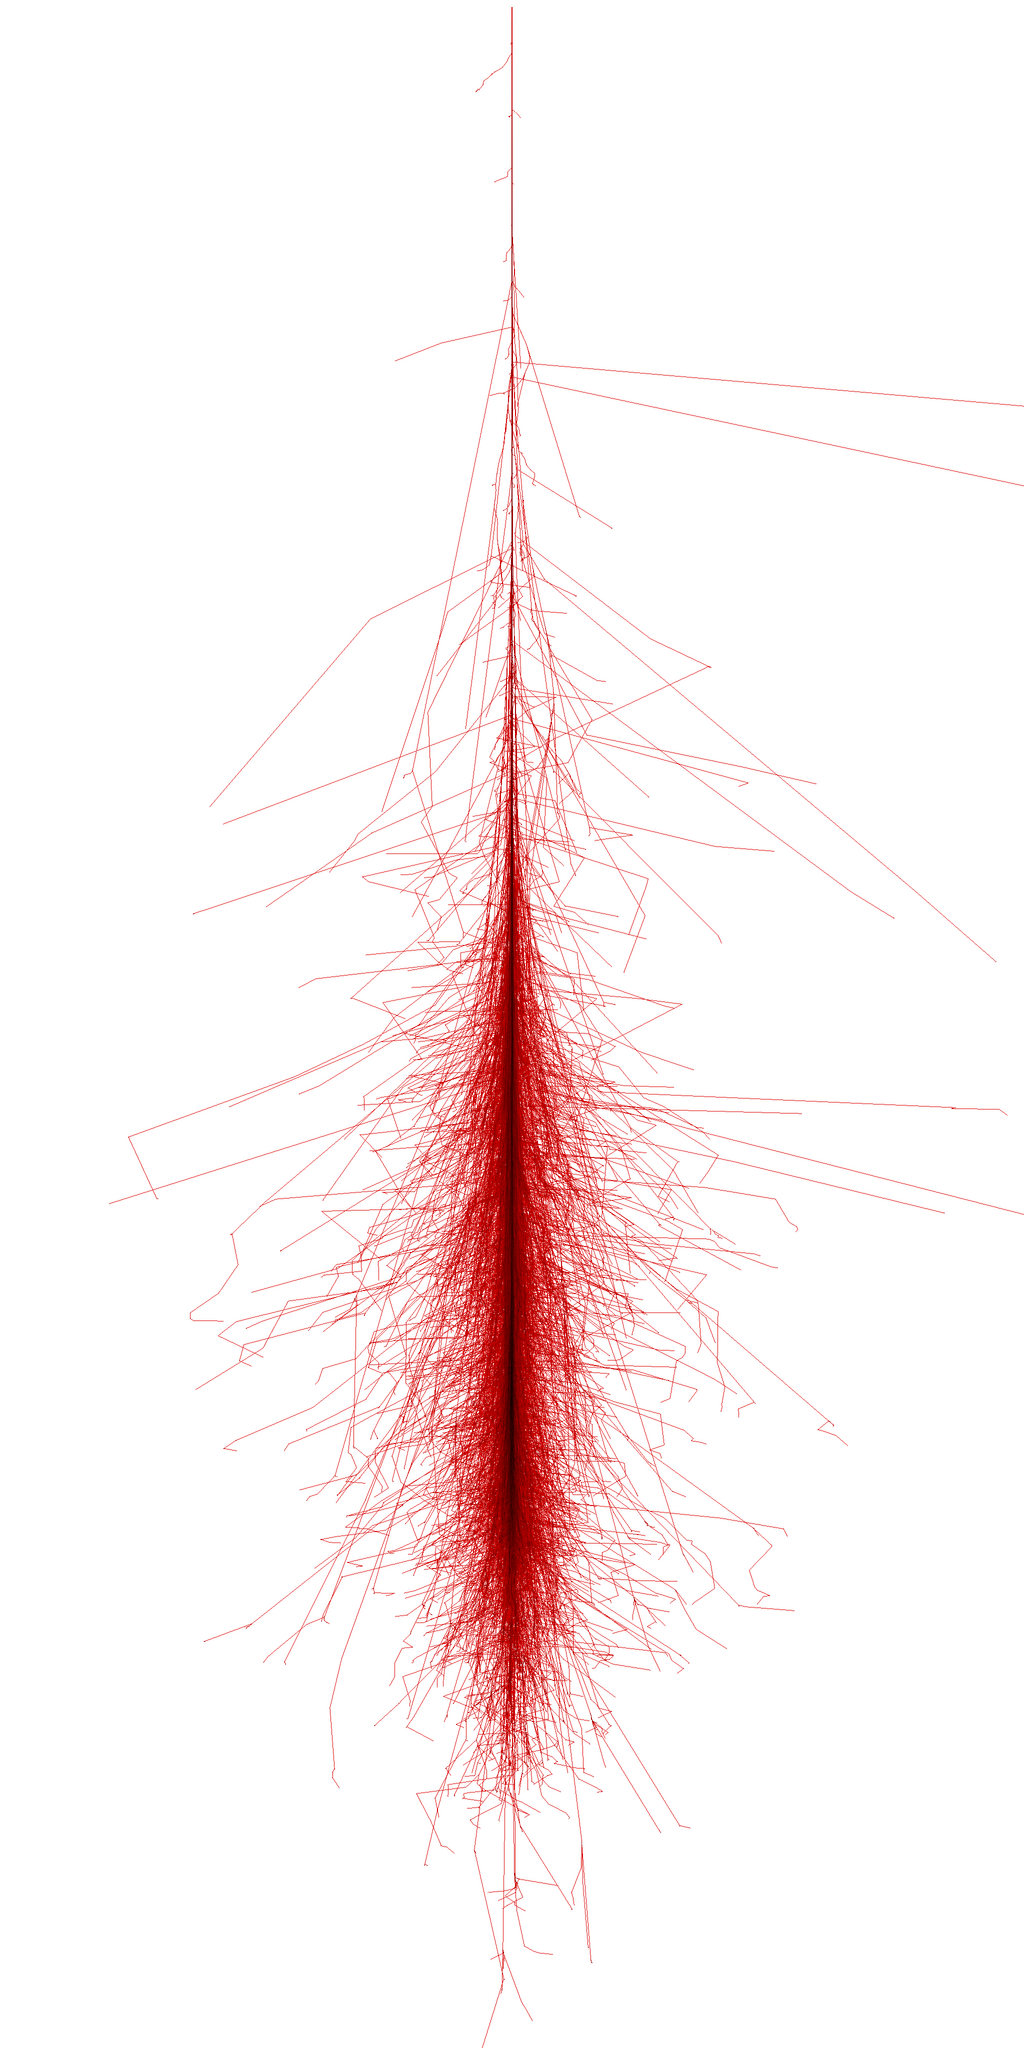
\includegraphics[width=0.5\textwidth]{images/photon_100GeV.png}
	\caption{Elektromagnetischer Schauer}
  \end{subfigure}
  \begin{subfigure}[t]{0.49\textwidth}
  	\centering
	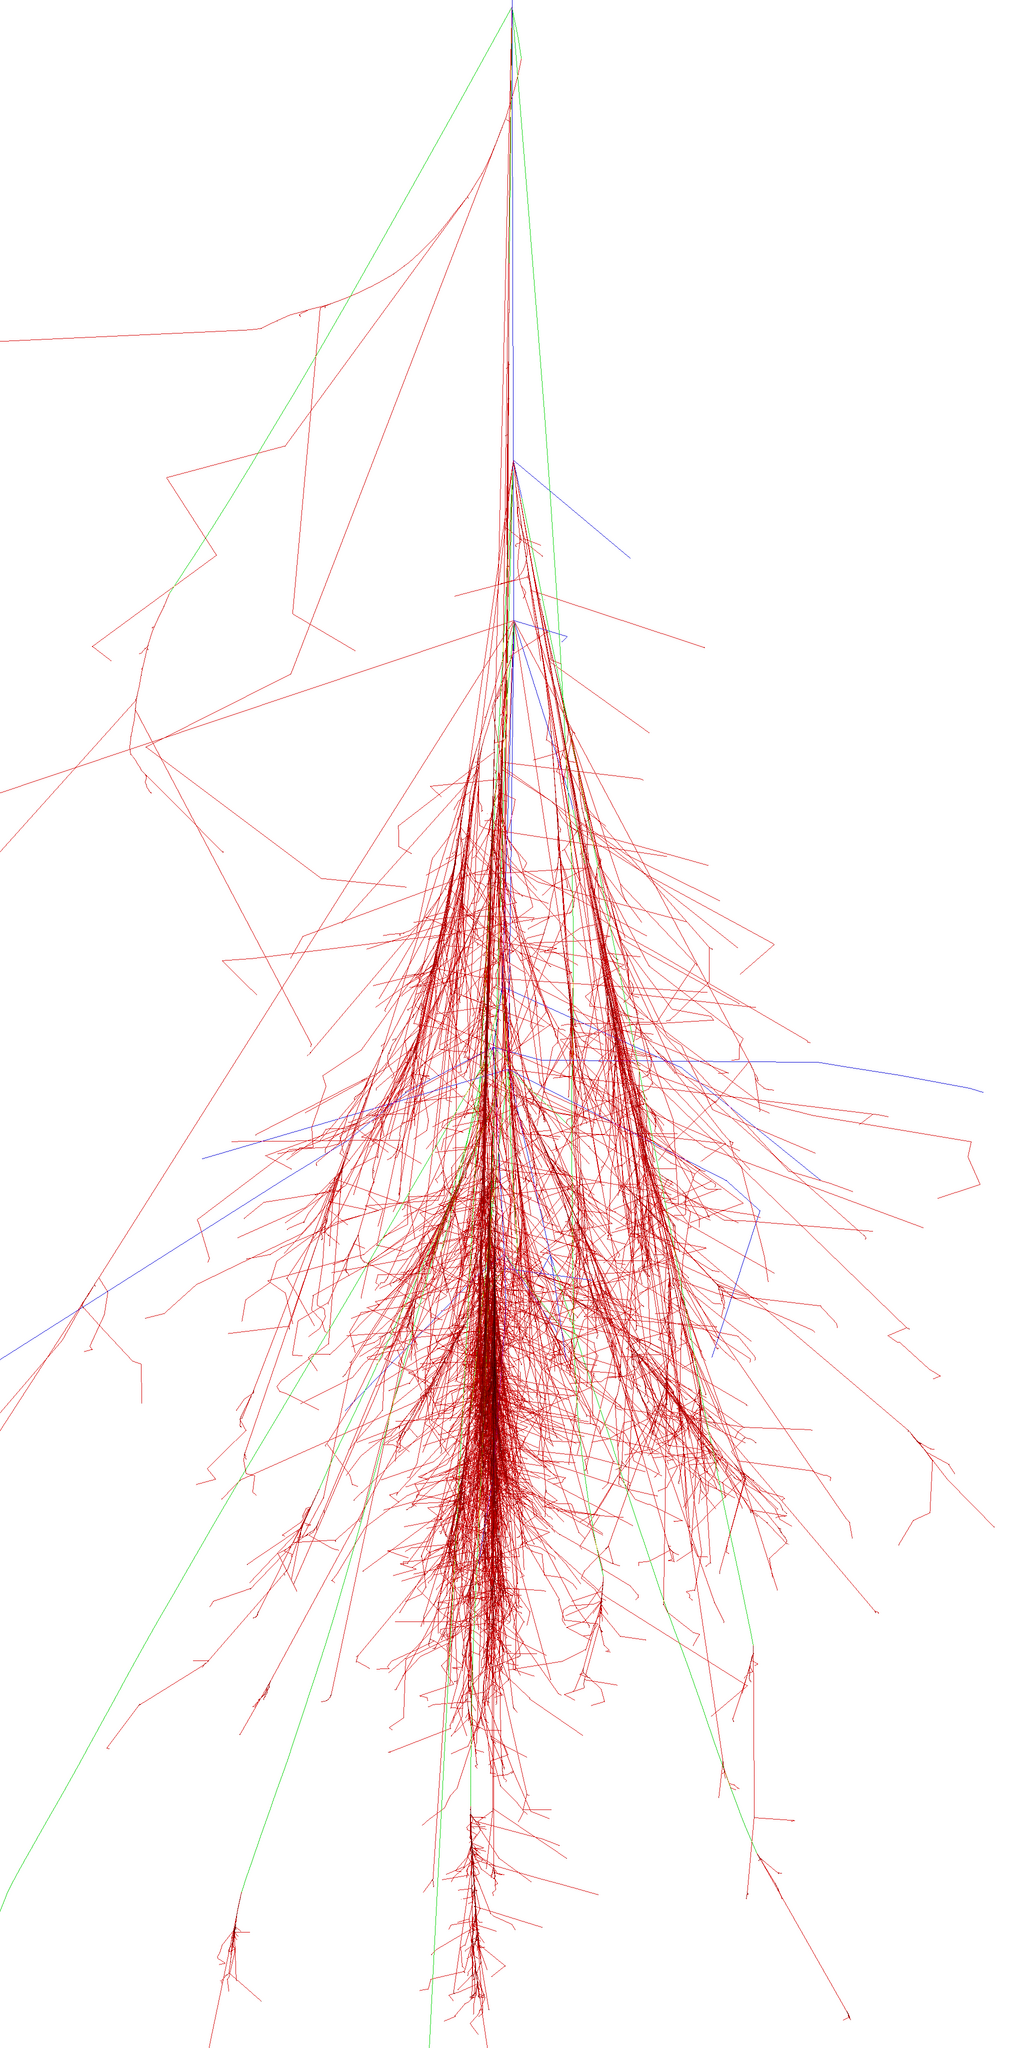
\includegraphics[width=0.5\textwidth]{images/proton_100GeV.png}
	\caption{Hadronischer Schauer}
  \end{subfigure}
  \caption{Simulierte Teilchenschauer mit einer Energie des Primärteilchens von \SI{100}{\giga \electronvolt} \cite{corsika}.}
\end{figure}
Trifft ein hochenergetisches $\gamma$-Quant auf die Atmosphäre, so wird es wahrscheinlich im Coulombwall der Moleküle durch Paarerzeugung ein Elektronen-Positron-Paar erzeugen. 
Anschließend kann bei hinreichend großer Energie das Elektron durch Bremsstrahlung weitere Photonen erzeugen. 
\begin{eqnarray}
  \gamma \rightarrow& e^{+} + e^{-} \\
  e^{+} \rightarrow& e^{+'} + \gamma \\
  e^{-} \rightarrow& e^{-'} + \gamma 
\end{eqnarray}
Dieser Prozess ist solange fortlaufend bis die Energie der Teilchen zu klein ist, um ein neues Teilchenpaar zu erzeugen und wird elektromagnetischer Schauer genannt.

Trifft ein geladenes kosmisches Teilchen in die Atmosphäre, so kann es über die starke Wechselwirkung, anders als beim elektromagnetischen Schauer, unterschiedliche Sekundärteilchen bilden. 
Dabei entstehen unter anderem neue Hadronen und Myonen, welche wiederum zerstrahlen. 
\begin{eqnarray}
  \pi^{0} \rightarrow& \gamma + \gamma \\
  \pi^{+} \rightarrow& \mu^{+} + \nu_{\mu} \\
  \pi^{-} \rightarrow& \mu^{-} + \bar{\nu}_{\mu}
\end{eqnarray}
Entsteht bei der Paarbildung schon früh ein $\pi^{0}$~Meson, so ist der hadronische Teilchenschauer kaum von dem eines $\gamma$-Quants zu unterscheiden. 

Bewegt sich ein Teilchen schneller als die Lichtgeschwindigkeit in dem Medium $c_\text{med}$, polarisiert es dieses kurzzeitig. 
Durch den Tscherenkow-Effekt wird eine kohärente Schockwelle in Bewegungsrichtung abgestrahlt. 
Diese bildet einen Mach-Kegel aus, dessen Öffungswinkel $\theta$ von dem Brechungsindex $n$ des Mediums und der Phasengeschwindigkeit der Welle $\beta = v / c_\text{0}$ abhängt.
\begin{equation}
  \cos  \theta = \frac{1}{\text{n} \beta}
\end{equation}
\chapter{Observation}
\section{Parametrisierung des Schauerbildes}
\begin{figure}[H]
  \centering
  \includegraphics[width=0.5\textwidth]{tikz/camera/camera.pdf}
  \caption{Parametrisierung des Kamerabildes durch Hillas-Parameter.}
\end{figure}
Die im Schauer entstehenden Tscherenkow-Photonen werden vom Teleskopspiegel in die Kamera reflektiert.
So entsteht in der Kamera ein Abbild des Schauers, das durch verschiedene Parameter beschrieben werden kann.
Diese Parameter bilden nachfolgend die Attribute, auf deren Basis ein maschineller Lerner den Schauer klassifiziert.
Nachdem Artefakte und äußere Einflüsse bereinigt worden sind, werden anhand der Pixel, die auf den Tscherenkow Schauer zurückzuführen sind, die Hillas-Parameter~\cite{hillas} berechnet. 
Dazu werden die Momente der Lichtverteilung bestimmt. 
Zu den Hillas-Parametern zählen:
\begin{itemize}
  \item \textbf{width/length:} Hauptachsen der Ellipse
  \item \textbf{size:} Anzahl an Photonen im Schauer
  \item \textbf{CoG:} Schwerpunkt des Schauers
%  \item \textbf{Source Position:} erwartete Quellposition
  \item \textbf{DISP:} Abstand zwischen Schwerpunkt des Schauers und der gemessenen Quellposition. Anhand der Parameter width und length wird DISP abgeschätzt, um die gemessene Quellposition zu ermitteln. Dabei gibt es zwei mögliche Vorzeichen, wobei über höhere Momente das korrekte Vorzeichen geschätzt wird.
  \item \textbf{$\theta$:} Winkel zwischen der gemessenen und echten Quellposition
\end{itemize}
\section{Wobble Observation-Strategie}
\begin{wrapfigure}[18]{L}[0pt]{0.53\textwidth}
  \includegraphics[width=0.5\textwidth]{tikz/wobble/wobble.pdf}
  \caption{Bestimmung von $\theta$ im Wobble Obersvationsmodus.}
\end{wrapfigure}
Zur Abschätzung der Untergrundstrahlung in der Quellregion (On-Position) werden Stellen am Himmel beobachtet, an denen keine Quellen zu erwarten sind (Off-Position).
Die gemessenen Untergrundraten können dann von den Messungen in der Quellregion subtrahiert werden, um die tatsächliche Signalrate zu bestimmen.
%Zur Bestimmung des Aktivität einer Quelle, werden bei deren Observation einerseits Daten aus der Quellregion (On-Position), sowie Daten aus ähnlichen Richtungen einer Position bei denen nur diffuse Hintergrundstrahlung (Off-Position) erwatet wird genommen. Aus der Beziehung der On- und Off-Daten wird versucht die statistische Effekte der Hintergrundstrahlung bei der Quellobservation zu minimieren.

Die Wobble Observation-Strategie zeichnet aus, dass nicht nacheinander On-/Off-Positionen beobachtet werden müssen. 
Stattdessen wird die erwartete Quellpostion \SI{0.6}{\degree} neben die Kameraachse gelegt. 
Dies hat zur Folge, dass es mehrere Positionen mit demselben Abstand und Symmetrie zur Kameraachse gibt. 
Bei der Standardanalyse von FACT können so neben der On-Position fünf Off-Positionen mit identischem Winkel zur Kameraachse gemessen werden. 
Somit ergibt sich für jeden Datensatz jeweils ein $\theta_\text{on}$ und fünf $\theta_\text{off}$. 
Für sehr kleine $\theta$ kann oftmals geschlossen werden, dass das gemessene Teilchen aus der Richtung der Quelle kam und vermutlich ein $\gamma$-Quant ist. 
Da der Hadronuntergrund isotrop in alle Richtungen verteilt auftritt, sollte bei hadronischen Schauern $\theta^{2}$ in etwa gleichverteilt sein. 
Zu den Vorteilen dieser Methode zählt, dass keine extra Off-Daten genommen werden müssen. 
Somit ist es möglich, die Messzeit zu maximieren. 
Des weiteren kann durch die simultane Datennahme davon ausgegangen werden, dass für die On/Off-Positionen dieselben Detektor- und Wetterbedingungen gelten. 

% \section{Events in der Kamera}
% 
% Dies liegt dem physikalischem Problem zugrunde, dass ein Proton, beim Eintritt in die Atmosphäre schon früh in ein $\pi^{0}$ Meson und einem $e^{+}$ zerfällt und kaum von einem elektromagnetischen Schauer zu unterscheiden ist.
% Dabei zerfällt das $\pi^{0}$ Meson in zwei Gamma-Teilchen, ebenso wie das $e^{+}$ durch inverse Bremsstrahlung weitere Gamma-Teilchen erzeugt. 
% Dies hat zur Folge, dass Proton- und Gamma-Schauer sehr ähnlich ausschauen können.
% \begin{figure}[H]
%   \centering
% \begin{subfigure}[t]{0.3\textwidth}
%   \centering
%   \includegraphics[width=\textwidth]{./images/Gamma.pdf}
%   \caption{Gamma Ereignis}
%   \label{fig:gammaevent}
% \end{subfigure}
% \begin{subfigure}[t]{0.3\textwidth}
%   \centering
%   \includegraphics[width=\textwidth]{./images/Hadron.pdf}
%   \caption{Hadron Ereignis mit Ähnlichkeit zu einem Gamma Ereignis}
%   \label{fig:hadevent}
% \end{subfigure}
% \begin{subfigure}[t]{0.3\textwidth}
%   \centering
%   \includegraphics[width=\textwidth]{./images/Hadron2.pdf}
%   \caption{Hadron Ereignis ohne Ähnlichkeit zu einem Gamma Ereignis}
%   \label{fig:had2event}
% \end{subfigure}
% \caption{Ereignisse in der Detektor Kamera vor dem Cleaning \cite{campic}}
% \label{fig:picevents}
% \end{figure}
% Der Anschaulichkeit halber sind in Abbildung~\ref{fig:picevents} drei Kamerabild zu sehen.
% Dabei weist das Proton Ereignis in Abbildung~\ref{fig:hadevent} eine Gewisse Ähnlichkeit zu dem Gamma Ereignis (Abbildung~\ref{fig:gammaevent}) auf, wohingegen das Ereignis in Abbildung~\ref{fig:had2event} wenig Ähnlichkeit aufweist.

\chapter{Überwachtes Maschinelles Lernen}
Zur Auswertung der Datenmenge von 300 GB bis 1 TB, die FACT jede Nacht aufnimmt, werden maschinelle Lernmethoden verwendet. 
Maschinelles Lernen kann dazu genutzt werden, Muster und Strukturen auf Datensätzen zu erkennen und zukünftige Ereignisse hervorzusagen. 
Dabei wird zwischen überwachtem und unüberwachtem Lernen unterschieden.

Unüberwachtes Lernen zeichnet sich dadurch aus, dass versucht wird, auf dem Trainingsdatensatz Muster zu erkennen. 
Hierbei werden keine Klassen vorgegeben, in die sich ein Datensatz aufteilen lässt. 
Der Lerner sucht eigenständig nach Strukturen, die für den Menschen nicht sichtbar sind.

Beim überwachten Lernen sind die Klassen, in die ein Datensatz unterteilt werden soll, bekannt.
Ziel ist es, bei einem gegebenen Trainingsset, welches aus Eingangsvariablen $X$ und Zielvariablen $y$ besteht, Modelle zu finden, welche $X$ bestmöglich auf $y$ abbilden. 
Zunächst muss das Modell trainiert werden. 
Dafür wird ein Datensatz, bei dem die Zielvariablen $y$ bekannt sind, in zwei Teile aufgeteilt, den Trainings- und den Testdatensatz. 
Dabei wird das Modell auf den Trainingsdatensatz optimiert und anschließend auf dem Testdatensatz evaluiert. 
Hier ist darauf zu achten, dass das Modell nicht nur den Trainingsdatensatz auswendig lernt (Übertraining), sondern allgemein genug bleibt, um auch ähnliche Datensätze genau vorherzusagen. 
Dies erfolgt durch Beschränkung der Modelle. 
Durch Berechnung von Evaluationsmetriken auf dem Testdatensatz, welcher unabhängig von dem Trainingsdatensatz ist, kann geprüft werden, ob das Modell allgemein genug ist oder an Übertraining leidet.
\section{Entscheidungsbaum}
\begin{wrapfigure}[13]{R}[0pt]{0.5\textwidth}
  \centering
  \includegraphics[width=0.5\textwidth]{./tikz/tree/tree.pdf}
  \caption{Entscheidungsbaum der Tiefe 2 für die Gamma/Handron-Separation.}
\end{wrapfigure}
Ein Entscheidungsbaum beginnt mit einem Wurzelknoten. Ausgehend von diesem wird durch Abfrage von verschiedenen Bedingungen eine Auswahl an Folgeknoten getroffen. 
In der Regel werden in der Datenanalyse binäre Entscheidungsbäume genutzt, da sich viele Probleme zu einem zwei-Klassen-Problem (Signal/Untergrund) reduzieren lassen.
% aufgrund dessen das sich jedes komplexeres auf ein binäres reduzieren lässt.
Entsprechend eines Schwellwertes wird der Datensatz aufgeteilt, sodass die entstehenden Untergruppen möglichst homogen werden. 
%sodass der Baum entsprechend an einem threshold wert die Daten an jedem Knoten in die zwei folgenden Knoten aufspaltet. 
%Dieser Prozess wird solange durchgeführt bis ein Blatt erreicht wird, in dem sich ausschließlich Ereignisse einer Klasse befinden und eine erneute Aufspaltung keinen Erkenntnissgewinn bringt. 
Dieser Prozess wird solange durchgeführt bis nach einer Abfrage alle Ereignisse ausschließlich einer Klasse angehören oder eine erneute Aufspaltung keinen Erkenntnissgewinn bringt. Die Enden einer solchen Abfrage werden als Blätter bezeichnet und geben die Vorhersage des Baumes an.
Die Anzahl an Knoten, die durchlaufen werden bis das letzte Blatt errreicht ist, wird als Tiefe der Bäume bezeichnet.
Der Baum kann entsprechend verschiedener Kriterien gebaut werden.
Zu den gängigen gehören die Entropie oder der Gini-Index \cite{model}. 
Zu den Vorteilen eines Entscheidungsbaums zählt, dass dieser gut interpretierbar und nachvollziehbar ist. 
Allerdings kommt es ohne Beschränkung schnell zum Übertraining.
\section{Random Forest}
Ein Random Forest besteht aus vielen unabhängigen Entscheidungsbäumen.
Jeder Entscheidungsbaum zieht bei der Erstellung immer nur eine Teilmenge aus allen Attributen.
Zur Klassifizierung wird anschließend eine Mehrheitsabstimmung über alle Entscheidungsbäume durchgeführt.
Dadurch, dass die einzelnen Bäume unterschiedlich aufgebaut sind und über die einzelnen Lerner gemittelt wird, ergibt sich ein Modell mit reduzierter Varianz im Gegensatz zum Entscheidungsbaum, welches resistenter gegen Übertraining ist.
\section{Extreme Gradient Boosting}
Extreme Gradient Boosting (kurz XGBoost) wurde von Jerome H. Friedman~\cite{xgboost} entwickelt.
XGBoosted Entscheidungsbäume zeichnen sich durch stark in der Tiefe beschränkte Bäume aus.
Anders als beim Random Forest werden nicht beliebig viele Bäume parallel gebaut, sondern iterativ. 
Dabei lernt der folgende Baum die Fehler, welche der vorherige Baum gemacht hat, zu minimieren.
Zusätzlich werden fehlklassifizierten Ereignissen der vorherigen Iteration höhere Gewichtungen zugewiesen.

\section{Evaluationsmetriken}
Um zu überprüfen, wie sich die Modelle auf Datensätzen verhalten, werden zweierlei Metriken zu der Beurteilung der Klassifizierer benutzt.
\subsection*{Receiver Operating Characteristic}
\begin{wrapfigure}[15]{R}[0pt]{0.45\textwidth}
  \centering
  \includegraphics[scale=1]{./Plots/roc_info.pdf}
  \caption{ROC-AUC-Wert zweier verschiedener Modelle}
  \label{fig:roc}
\end{wrapfigure}
Zum Vergleich von verschiedenen binären Klassifizierern ist die \enquote{Receiver Operating Characteristic Curve} ein Maß für die Güte der Separation. 
Dafür wird zunächst der Konfidenzwert des Klassifizierers berechnet. 
Dies ist ein Wert zwischen 0 und 1, welcher die Sicherheit wiederspiegelt, dass die Vorhersage den Zielklassen 0 oder 1 entspricht.
Für alle möglichen Konfidenzwerte wird der prozentuale Anteil an richtig klassifizierten Ereignissen der Klasse 1 (true positive rate, TPR) und an falsch klassifizierten der Klasse 0 (false positive rate, FPR) berechnet. 
Bei der ROC Curve wird die TPR gegen die FPR aufgetragen. 
Ein Beispiel ist in Abbildung~\ref{fig:roc} zu sehen.
Für einen guten Klassifizier strebt die Kurve bei kleinen FPR gegen hohe TPR. 
Ist der Klassifizierer nicht in der Lage zwischen den beiden Klassen zu separieren, steigen die TPR und FPR gleichermaßen. 
Anhand der Fläche unter der Kurve kann die Güte verglichen werden.
\subsection*{Signifikanz nach Li und Ma}
% Aufgrund der Begrenztheit der Dektorsensitivität muss bei der Analyse von möglichen Quellen sorgsam mit den Daten zur Bestimmung der Sicherheit einer Quelle umgegangen werden.
% Dabei kann nicht das Signal einer Quelle isoliert gemessen werden. 
% Stattdessen muss eine Sicherheit auf das Signals welches aus Richtung der Quelle $N_\text{on}$ und des Hintergrunds $N_\text{off}$ gegeben werden, dass das gemessene Signal nicht nur statistisches Rauschen ist.
Signal und Untergrund sind schwer zu unterscheiden, da das Signal oftmals wesentlich schwächer als der Untergrund ist und nicht isoliert gemessen werden kann. 
Daher wird ein Maß für die statistische Sicherheit angegeben, mit der es sich bei einem gemessenen Signal tatsächlich um eine Quelle und nicht um statistisches Rauschen handelt.
Ein möglicher Anatz ist die Li und Ma Signifikanz \cite{liandma}, bei der über einen statistischen Hypothesentest geprüft wird, ob das Signal nur ein Teil des Untergrunds ist. 
Aus dem Verhältnis der Messzeiten der On- und Off-Position $\alpha$ wird die Hintergrundstrahlung berechnet. 
Aus der Differenz der Anzahl an Ereignissen in der On-Region und der Hintergrundrate lässt sich die Signalrate bestimmen. 
Durch das Aufstellen der Maximum Likelihood Funktion und des anschließenden Tests ergibt sich für die Signifikanz nach Li und Ma
\begin{equation}
S = \sqrt{2} \left( N_\text{on} \ln \left[ \frac{1+ \alpha}{\alpha}\left( \frac{N_\text{on}}{N_\text{on} + N_\text{off}} \right) \right] + N_\text{off} \ln \left[ \left( 1+ \alpha \right) \left( \frac{N_\text{off}}{N_\text{on} + N_\text{off}} \right) \right] \right)^{1/2},
\end{equation}
wobei $N_\text{on}$ die Anzahl gemessener Ereignisse in der On-Region angibt und $N_\text{off}$ entsprechend in der Off-Region.

\chapter{Untersuchte Quellen}
In dieser Arbeit werden Datensätze von zwei verschiedenen Quellen verwendet. 
Beide Quellen sind bereits gut verstanden und können zum Vergleich mit anderen Arbeiten verwendet werden.
\section{Krebsnebel}
In einer Entfernung von 6400 Lichtjahren befindet sich im Sternzeichen Stier der Überrest der ersten dokumentierten Supernovaexplosion, die auf das Jahr 1054 datiert ist. 
Die Überreste erstrecken sich über eine Fläche von 6 Bogenminuten Länge und 4 Bogenminuten Breite. 
In der Mitte des Krebsnebels liegt ein Pulsar, welcher sich bei einem Durchmesser von etwa \SI{30}{\kilo \meter} 30 mal pro Sekunde um seine eigene Achse dreht.
Der Pulsar emittiert regelmäßige Gammastrahlungspulse, wodurch der Krebsnebel eine Standard- und Kalibrierungsquelle in der Gammaastronomie ist.
Viele wissentschaftliche Arbeiten nehmen ihn als Referenzwert, um ihre Messwerte zu vergleichen. 

\section{Markarian 501}
Im Sternbild Herkules befindet sich in einer Entfernung von etwa 500 Millionen Lichtjahren der Blazar Markarian 501. 
In seinem Zentrum befindet sich ein \num{0.9} bis \num{3.4} Milliarden Sonnenmassen schweres schwarzes Loch, dessen Jet in Richtung Erde gerichtet ist.
Auch dieser gilt als eine der stärksten Gammastrahlungsquellen.
